\documentclass[conference]{IEEEtran}
\IEEEoverridecommandlockouts
\usepackage{cite}
\usepackage{amsmath,amssymb,amsfonts,amsthm}
\usepackage{algorithmic}
\usepackage{algorithm}
\usepackage{graphicx}
\usepackage{textcomp}
\usepackage{xcolor}
\usepackage{booktabs}
\usepackage{hyperref}
\usepackage{tikz}
\usepackage{multirow}
\usepackage{enumitem}
\usetikzlibrary{shapes.geometric, arrows.meta, positioning, fit, calc, backgrounds, patterns}

\newtheorem{theorem}{Theorem}
\newtheorem{lemma}[theorem]{Lemma}
\newtheorem{definition}{Definition}

\def\BibTeX{{\rm B\kern-.05em{\sc i\kern-.025em b}\kern-.08em
    T\kern-.1667em\lower.7ex\hbox{E}\kern-.125emX}}

\begin{document}

\title{FAMM: Future-Aware Adaptive Memory Management Framework for Long-Term Autonomous LLM Agents}

\author{
\IEEEauthorblockN{Suyash Vakhariya and Asmita Ipper}
\IEEEauthorblockA{Department of Computer Engineering \\
PDEA College of Engineering \\
Savitribai Phule Pune University \\
Pune, Maharashtra, India \\
vakhariyasuyash@gmail.com \\ asmitaipper@gmail.com}
}

\maketitle

\begin{abstract}
As Large Language Model (LLM) agents are increasingly deployed for long-term, unbounded operational tasks, managing their finite context windows becomes a critical architectural bottleneck. Existing Retrieval-Augmented Generation (RAG) and episodic memory systems typically rely on reactive heuristics---such as raw semantic similarity, uniform temporal decay, or static importance scoring---to determine which context to retain. These approaches fail in high-noise, temporally extended workflows due to context pollution and retrieval noise. We introduce the Future-Aware Adaptive Memory Management (FAMM) framework, an architecture that proactively estimates the future operational utility of each memory at write time. FAMM employs a lightweight, deterministic feature-based scoring function that bypasses LLM evaluation calls and drives a utility-conditioned decay mechanism coupled with a four-signal composite retrieval ranker incorporating semantic similarity, predicted utility, goal alignment, and temporal recency. We evaluate FAMM against four baseline architectures---Similarity-Only RAG, Importance Scoring, Uniform Ebbinghaus Decay, and FIFO eviction---on a synthetic research agent dataset scaled to 10,000 vector memories. Our results reveal a nuanced finding: while FAMM's write-path architecture achieves effective storage consolidation and low-latency prediction without LLM calls, its goal-alignment retrieval signal introduces systematic over-filtering that degrades recall at all tested scales (NDCG@10 of 0.494 at $N{=}10{,}000$ vs.\ 0.750 for Importance Scoring). Ablation confirms that disabling goal-alignment restores competitive retrieval performance, providing a cautionary empirical result regarding multi-signal ranking in dense embedding spaces.
\end{abstract}

\begin{IEEEkeywords}
Large Language Models, Retrieval-Augmented Generation, Autonomous Agents, Vector Databases, Memory Management, Semantic Search, Complexity Analysis
\end{IEEEkeywords}

%% ============================================================
%% SECTION 1: INTRODUCTION
%% ============================================================
\section{Introduction}
\label{sec:intro}

\subsection{Motivation and the Rise of Autonomous Agents}
The architectural maturation of Large Language Models (LLMs) has catalyzed a paradigm shift in artificial intelligence. Historically utilized as stateless text generators \cite{zhao2023survey}, contemporary LLMs increasingly serve as the cognitive reasoning engines for autonomous, goal-directed agents. These agents execute complex, multi-step workflows across software engineering, scientific research, and enterprise operations \cite{wang2023survey}.

A defining characteristic of these deployments is temporal persistence. Unlike traditional zero-shot query systems, modern autonomous agents must maintain a coherent, evolving internal state across interactions spanning days or months. This requirement mirrors the operational realities of human cognitive systems, where contextual continuity is essential for trust, efficiency, and task resolution. However, the foundational architecture of transformer-based LLMs imposes a hard constraint on this autonomy: the finite context window.

\subsection{The Bottleneck of Finite Context Windows}
Transformer architectures rely on self-attention mechanisms with quadratic computational cost $O(N^2 \cdot d)$ with respect to sequence length $N$ and model dimension $d$ \cite{vaswani2017attention, ding2024longcontext}. Although engineering advances such as Ring Attention and sparse retrieval heads have expanded these boundaries to accommodate multi-million token windows, empirical evidence reveals persistent practical limitations. Injecting massive, unbounded operational histories into a static context window produces severe latency degradation.

Long-context models consistently exhibit the ``lost in the middle'' phenomenon: when critical instructions or operational constraints are buried within large blocks of noisy context, the attention mechanism fails to route them to the active reasoning stream. True long-term autonomy therefore cannot rely on brute-force context scaling; it requires structured, dynamic working memory architectures that selectively page critical information into the prompt space when the reasoning process demands it.

\subsection{Limitations of Current Retrieval-Augmented Generation}
Retrieval-Augmented Generation (RAG) \cite{lewis2020retrieval} has emerged as the standard approach for managing external knowledge without continuous model fine-tuning. Dense embeddings project historical events into high-dimensional vector spaces, enabling agents to query external vector databases \cite{johnson2019billion} for relevant context.

Despite its effectiveness in static, open-domain question-answering settings, traditional RAG rapidly deteriorates when applied to continuous, dynamic agent memory \cite{gao2023retrieval}. An autonomous agent's memory stream is not a pristine encyclopedic corpus; it quickly fills with redundant observations, transient API failure responses, ephemeral thought traces, and obsolete operational plans.

Traditional RAG retrieves memories based purely on the cosine similarity between the query embedding and stored vectors \cite{karpukhin2020dense}. In complex agentic workflows, however, high semantic similarity does not imply operational utility. An agent attempting to resolve a novel compiler error might retrieve thousands of semantically similar but practically useless logs of previous successful compilations. This naive semantic fetching produces context pollution and cascading hallucination loops \cite{mallen2023trust}.

\subsection{The Need for Proactive Adaptive Memory}
Recent cognitive architectures have introduced structural memory management to mitigate RAG failures. Frameworks such as Generative Agents \cite{park2023generative} and MemGPT \cite{packer2023memgpt} attempt to filter noise by utilizing uniform temporal forgetting curves or assigning static importance metadata at creation time.

While these architectures represent meaningful advances, they remain fundamentally reactive and often computationally expensive. Relying on the LLM itself to assign importance scores to every incoming observation requires secondary inference calls that dominate the agent's computational budget \cite{xu2023llm}. Moreover, static importance is highly contextual: a database password logged on day one is critically important until it is revoked on day two, at which point its importance should plummet---yet standard systems permanently shield it from eviction based on its initial high score.

Systems utilizing uniform forgetting curves introduce a complementary failure: they arbitrarily delete critical configuration data simply because it is chronologically old, treating a vital architectural constraint with the same temporal hostility as a transient web-scraping error. The field currently lacks an automated mechanism to decouple the chronological age of a memory from its operational utility.

\subsection{Research Contributions}
We hypothesize that memory management must transition from a reactive retrieval constraint to a proactive, write-time prediction. If an agent can estimate the \textit{future operational utility} of a memory at the moment of creation---using lightweight deterministic scoring rather than expensive LLM evaluations---it can autonomously structure its own forgetting curve.

To test this hypothesis, we introduce the \textbf{Future-Aware Adaptive Memory Management (FAMM)} framework. FAMM intercepts the memory write stream using a deterministic weighted feature scorer to estimate future utility from five predictive signals: goal similarity, recency, access frequency, source type prior, and entity overlap. This score drives a utility-conditioned decay mechanism that shields high-value memories from chronological eviction, and acts as a signal within a four-component composite retrieval ranker.

Our contributions are:
\begin{enumerate}
    \item We formulate the FAMM architecture, detailing an in-process observer-pattern event bus that decouples memory management from the LLM's primary reasoning loop, integrating write-time utility prediction and Union-Find background consolidation.
    \item We introduce a utility-conditioned discrete decay rule where the effective decay rate is inversely proportional to predicted utility, providing up to $81\times$ differential temporal shielding between high- and low-utility memories.
    \item We construct a four-signal composite retrieval ranker that synthesizes semantic similarity, predicted utility, goal alignment, and temporal recency into a unified ranking score.
    \item We provide empirical evaluation on a synthetic dataset scaled to $N{=}10{,}000$ dense vectors. Through ablation studies and complexity analysis, we document a cautionary finding: the goal-alignment signal introduces systematic over-filtering that degrades recall at all tested scales, while the write-path architecture (utility prediction, decay, consolidation) operates as designed.
\end{enumerate}

%% ============================================================
%% SECTION 2: BACKGROUND
%% ============================================================
\section{Background}
\label{sec:background}

This section provides foundational concepts necessary to contextualize FAMM within the broader landscape of LLM memory management.

\subsection{Transformer Memory and Context Windows}
The transformer architecture \cite{vaswani2017attention} processes input as a fixed-length token sequence. The self-attention mechanism computes pairwise relationships across all positions with cost $O(N^2 \cdot d)$ where $N$ is sequence length and $d$ is model dimension. This fixed sequence constitutes the model's \textit{working memory}: only information physically present within the current token buffer is accessible to the reasoning process.

\subsection{Working Memory vs.\ Long-Term Memory}
Drawing from cognitive science \cite{sumers2023cognitive}, agent memory architectures distinguish between \textit{working memory} (the active context window) and \textit{long-term memory} (persistent external storage). Working memory is fast but severely capacity-constrained. Long-term memory offers unbounded capacity but introduces retrieval latency and noise. The fundamental challenge is bridging these tiers efficiently---paging critical data from long-term storage into working memory exactly when the reasoning process requires it.

\subsection{Dense Embeddings and Vector Databases}
Dense embedding models project variable-length text strings into fixed-dimensional vector spaces. Models such as \texttt{all-MiniLM-L6-v2} \cite{reimers2019sbert} produce 384-dimensional L2-normalized vectors where geometric proximity corresponds to semantic similarity. Vector databases (e.g., ChromaDB, FAISS) maintain these embeddings in specialized indices---typically Hierarchical Navigable Small World (HNSW) graphs \cite{malkov2018hnsw}---that support approximate nearest neighbor (ANN) search in $O(\log N)$ time. The combination of dense embeddings with ANN indices forms the backbone of modern RAG systems.

%% ============================================================
%% SECTION 3: RELATED WORK
%% ============================================================
\section{Related Work}
\label{sec:related}

\subsection{LLM-Dependent Memory Architectures}
\textbf{Generative Agents} \cite{park2023generative} introduced a three-signal retrieval function combining recency, importance, and relevance. However, the importance score requires a full LLM inference call for every stored observation, creating a write-path bottleneck that scales linearly with memory volume.

\textbf{MemGPT} \cite{packer2023memgpt} models LLM memory management as an operating system, implementing virtual paging between a fixed main context and an unbounded archival store. Every page-in/page-out operation requires an LLM function call, introducing latency proportional to the frequency of context switches.

\textbf{Reflexion} \cite{shinn2023reflexion} maintains episodic failure logs that the agent consults to avoid repeating mistakes. This approach excels at short-horizon error correction but provides no mechanism for long-term memory management or temporal decay.

\textbf{Self-RAG} \cite{asai2023selfrag} augments generation with self-reflective critique tokens that assess retrieval quality. While this improves generation fidelity, it adds inference overhead at every generation step and does not address the upstream problem of memory organization.

\subsection{Memory Decay and Consolidation Systems}
\textbf{MemoryBank} \cite{zhong2023memorybank} applies the Ebbinghaus forgetting curve to LLM memory, implementing a uniform exponential decay across all stored records. Because this decay is content-agnostic, it arbitrarily evicts critical configuration data that happens to be chronologically old.

\textbf{A-MEM} \cite{zheng2025amem} treats memories as self-organizing ``Zettelkasten'' notes where the agent creates and links memory entries. While this approach excels at organic knowledge structuring, every memory operation requires a full LLM call, limiting throughput to the rate of the underlying language model.

\subsection{Advanced Retrieval Architectures}
\textbf{GraphRAG} \cite{edge2024graphrag} builds knowledge graphs from document collections, enabling entity-relation traversal queries. The graph construction phase, however, requires extensive LLM extraction calls and does not support the real-time write throughput needed for continuous agent memory streams.

\textbf{HippoRAG} \cite{guan2024hipporag} mimics hippocampal indexing by maintaining a knowledge graph alongside dense vectors. The dual-index approach provides superior recall on knowledge-intensive benchmarks but introduces significant indexing overhead incompatible with high-velocity agentic data.

\textbf{RAPTOR} \cite{sarthi2024raptor} constructs hierarchical cluster trees over document collections, enabling multi-level summarization retrieval. Each tree construction step requires LLM-based summarization, making the approach computationally prohibitive for streaming memory contexts.

\subsection{Lightweight Memory Systems}
\textbf{LongMem} \cite{wang2023longmem} augments language models with a side-network memory module that caches recent activations. \textbf{LightMem} \cite{luo2023lightmem} injects retrieved context via cross-attention mechanisms. Both approaches embed memory into the model's internal representations, sacrificing the auditability and transparency required for deployable autonomous systems.

\subsection{How FAMM Differs}
FAMM diverges from these paradigms by shifting memory management from a reactive retrieval constraint to a proactive, write-time prediction. Unlike MemGPT or Generative Agents, FAMM entirely removes the cognitive load of memory maintenance from the LLM, relying instead on a deterministic weighted scorer to predict utility. Unlike MemoryBank, FAMM's temporal decay is not uniform; it is conditioned on predicted utility. Unlike GraphRAG, RAPTOR, and HippoRAG, FAMM operates on flat vector spaces with lightweight Union-Find clustering. Unlike LightMem and LongMem, FAMM's memories remain fully discrete, transparent, and auditable. Table~\ref{tab:system_comparison} provides a structured comparison.

\begin{table*}[htbp]
\caption{Comparative Analysis of Memory Architectures for LLM Agents}
\label{tab:system_comparison}
\begin{center}
\small
\begin{tabular}{lccccc}
\toprule
\textbf{System} & \textbf{Memory Strategy} & \textbf{LLM Calls for Mgmt} & \textbf{Temporal Decay} & \textbf{Write Latency} & \textbf{Auditable} \\
\midrule
MemGPT \cite{packer2023memgpt} & OS-style paging & Yes (every page) & None & $>$2000 ms & Yes \\
Gen.\ Agents \cite{park2023generative} & Recency+Importance & Yes (every write) & Uniform & $>$2000 ms & Yes \\
MemoryBank \cite{zhong2023memorybank} & Ebbinghaus decay & Partial & Uniform & $\sim$500 ms & Yes \\
Reflexion \cite{shinn2023reflexion} & Failure episodic & Yes (reflection) & None & $>$2000 ms & Yes \\
Self-RAG \cite{asai2023selfrag} & Critique tokens & Yes (critique) & None & $>$1500 ms & Partial \\
GraphRAG \cite{edge2024graphrag} & Knowledge graph & Yes (extraction) & None & $>$5000 ms & Yes \\
HippoRAG \cite{guan2024hipporag} & Hippocampal graph & Yes (indexing) & None & $>$3000 ms & Yes \\
RAPTOR \cite{sarthi2024raptor} & Hierarchical tree & Yes (summarize) & None & $>$3000 ms & Yes \\
LongMem \cite{wang2023longmem} & Side-network cache & No & Implicit drift & $<$10 ms & No \\
LightMem \cite{luo2023lightmem} & Cross-attention inject & No & Implicit drift & $<$10 ms & No \\
A-MEM \cite{zheng2025amem} & Self-organizing notes & Yes (create+link) & None & $>$2000 ms & Yes \\
\midrule
\textbf{FAMM (Ours)} & \textbf{Predictive utility} & \textbf{No} & \textbf{Utility-conditioned} & \textbf{Sub-ms (scorer)} & \textbf{Yes} \\
\bottomrule
\end{tabular}
\end{center}
\end{table*}

%% ============================================================
%% SECTION 4: PROBLEM STATEMENT
%% ============================================================
\section{Problem Statement}
\label{sec:problem}

\begin{definition}[Agent Memory Record]
A memory record is a tuple $M = (s, t_0, \vec{v}, u)$ where $s \in \Sigma^*$ is the raw text string, $t_0 \in \mathbb{R}^+$ is the creation timestamp, $\vec{v} \in \mathbb{R}^d$ is the dense embedding vector, and $u \in [0,1]$ is a metadata scalar representing predicted utility.
\end{definition}

\begin{definition}[Memory Database]
The memory database $\mathcal{D} = \{M_1, M_2, \ldots, M_N\}$ is an ordered collection of $N$ memory records accumulated over the agent's operational lifetime.
\end{definition}

\textbf{Inputs.} At each reasoning step, the agent produces a new observation string $s_{new}$ and may issue a retrieval query $q$ conditioned on an active operational goal $g$.

\textbf{Outputs.} The system must (i) assign a predicted future utility $U(M) \in [0,1]$ to every incoming memory at write time, and (ii) return an ordered list $L = [M_{\pi(1)}, \ldots, M_{\pi(k)}]$ of the top-$k$ most operationally relevant memories for prompt injection.

\textbf{Optimization Objective.} The retrieval function $F$ must maximize recall:
\begin{equation}
\label{eq:objective}
\max_{F} \; \text{Recall@}k = \frac{|L \cap \mathcal{R}|}{|\mathcal{R}|}
\end{equation}
where $\mathcal{R} \subseteq \mathcal{D}$ denotes the ground-truth relevant memories for query $q$.

\textbf{Constraints.} (C1) Write-time utility prediction must execute in $O(1)$ time with respect to $N$. (C2) Retrieval must operate within $O(N \cdot d)$ time in the worst case. (C3) All stored memories must remain discrete, human-readable text.

%% ============================================================
%% SECTION 5: RESEARCH GAP
%% ============================================================
\section{Research Gap}
\label{sec:gap}
Despite the proliferation of the aforementioned systems, a critical gap remains at the intersection of dense vector scaling and automated memory eviction.

Systems that utilize \textit{static importance} fail because importance is contextual; a credential logged on day one is critical until revoked on day two, yet standard systems maintain its high score indefinitely. Systems relying on \textit{semantic retrieval alone} fail due to the geometry of dense embedding spaces; operational logs occupy tight clusters in vector space, causing retrieval noise where thousands of vectors collide. Systems utilizing \textit{uniform forgetting} fail because they delete critical configuration data simply because it is old. Systems utilizing \textit{graph-based indexing} fail because they cannot sustain real-time write throughput for high-velocity agentic data streams.

FAMM addresses this gap by making the temporal decay rate a function of predicted utility. High-utility memories receive slower decay; low-utility noise decays rapidly. This decoupling of chronological age from operational importance is the core contribution.

%% ============================================================
%% SECTION 6: DESIGN OBJECTIVES
%% ============================================================
\section{Design Objectives}
\label{sec:objectives}

The FAMM architecture satisfies six engineering requirements derived from the identified gap:

\begin{enumerate}[label=\textbf{O\arabic*.}, leftmargin=*]
    \item \textbf{Zero LLM overhead for memory management.} No secondary LLM inference calls for utility scoring, importance grading, or memory organization.
    \item \textbf{Deterministic, sub-millisecond write-path scoring.} The utility prediction pipeline must execute as a constant-time deterministic function.
    \item \textbf{Utility-conditioned temporal decay.} Critical memories must be mathematically shielded from chronological eviction based on their predicted utility.
    \item \textbf{Multi-signal retrieval.} The retrieval ranker must incorporate the agent's active goal as a ranking signal alongside semantic similarity, predicted utility, and recency.
    \item \textbf{Asynchronous deduplication.} Redundant memory trajectories must be automatically consolidated without blocking retrieval.
    \item \textbf{Full auditability.} All stored memories must remain discrete, human-readable text amenable to manual inspection and deletion.
\end{enumerate}

%% ============================================================
%% SECTION 7: PROPOSED FRAMEWORK
%% ============================================================
\section{Proposed Framework}
\label{sec:framework}

FAMM addresses the identified gap through a three-stage pipeline that operates entirely outside the LLM's token budget:

\textbf{Stage 1: Predictive Write Path.} When the agent produces a new observation, the text is intercepted by a deterministic feature scorer that extracts five predictive signals: goal similarity, recency, access frequency, source type prior, and entity overlap. These features are combined via a weighted linear function to produce a normalized utility prediction $U(M) \in [0,1]$. This score is attached as metadata before persistence.

\textbf{Stage 2: Utility-Conditioned Storage.} The predicted utility modulates a discrete decay parameter, creating a per-memory forgetting curve. High-utility memories receive slower decay, while low-utility noise decays rapidly. An asynchronous Union-Find consolidator periodically merges near-duplicate vectors in the background.

\textbf{Stage 3: Multi-Signal Retrieval.} At query time, the retrieval engine computes a composite ranking score fusing four independent signals: semantic similarity to the query, predicted utility, alignment to the agent's active goal, and temporal recency. The top-$k$ memories are injected into the LLM's system prompt.

Figure~\ref{fig:lifecycle} illustrates the complete memory lifecycle.

\begin{figure}[htbp]
\centering
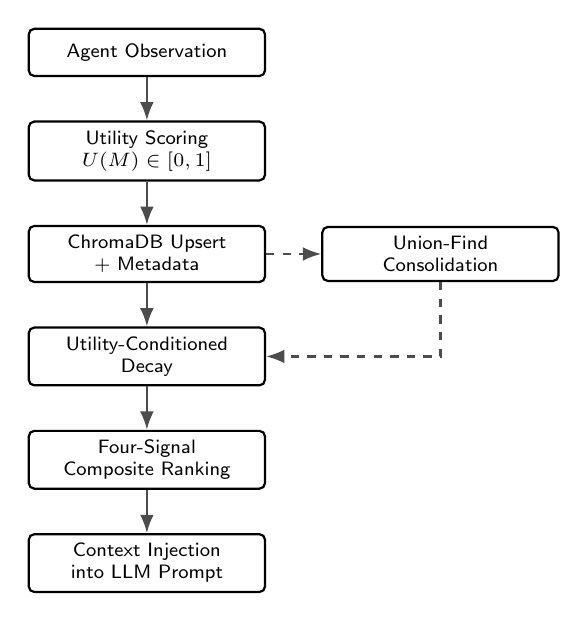
\begin{tikzpicture}[
    node distance=0.55cm,
    stage/.style={draw, rectangle, rounded corners=2pt, minimum width=3.0cm, minimum height=0.6cm, align=center, font=\scriptsize\sffamily, thick, fill=white},
    arrow/.style={-Latex, thick, draw=black!70}
]
\node[stage] (obs) {Agent Observation};
\node[stage, below=of obs] (pred) {Utility Scoring\\ $U(M) \in [0,1]$};
\node[stage, below=of pred] (store) {ChromaDB Upsert\\ + Metadata};
\node[stage, below=of store] (decay) {Utility-Conditioned\\ Decay};
\node[stage, below=of decay] (retrieve) {Four-Signal\\ Composite Ranking};
\node[stage, below=of retrieve] (inject) {Context Injection\\ into LLM Prompt};

\draw[arrow] (obs) -- (pred);
\draw[arrow] (pred) -- (store);
\draw[arrow] (store) -- (decay);
\draw[arrow] (decay) -- (retrieve);
\draw[arrow] (retrieve) -- (inject);

% Consolidator side branch
\node[stage, right=0.7cm of store, text width=1.8cm, font=\scriptsize\sffamily] (consol) {Union-Find\\ Consolidation};
\draw[arrow, dashed] (store.east) -- (consol.west);
\draw[arrow, dashed] (consol.south) |- (decay.east);

\end{tikzpicture}
\caption{FAMM memory lifecycle. Observations pass through utility scoring, storage with conditioned decay, and multi-signal retrieval. The Union-Find consolidator operates asynchronously.}
\label{fig:lifecycle}
\end{figure}

%% ============================================================
%% SECTION 8: SYSTEM ARCHITECTURE
%% ============================================================
\section{System Architecture}
\label{sec:architecture}

The FAMM architecture is designed to resolve the conflict between continuous autonomous operation and the I/O latency introduced by external vector databases. The architecture is strictly decoupled: the primary LLM reasoning loop is never blocked by memory maintenance routines. Figure~\ref{fig:arch} presents the system topology.

\begin{figure*}[htbp]
\centering
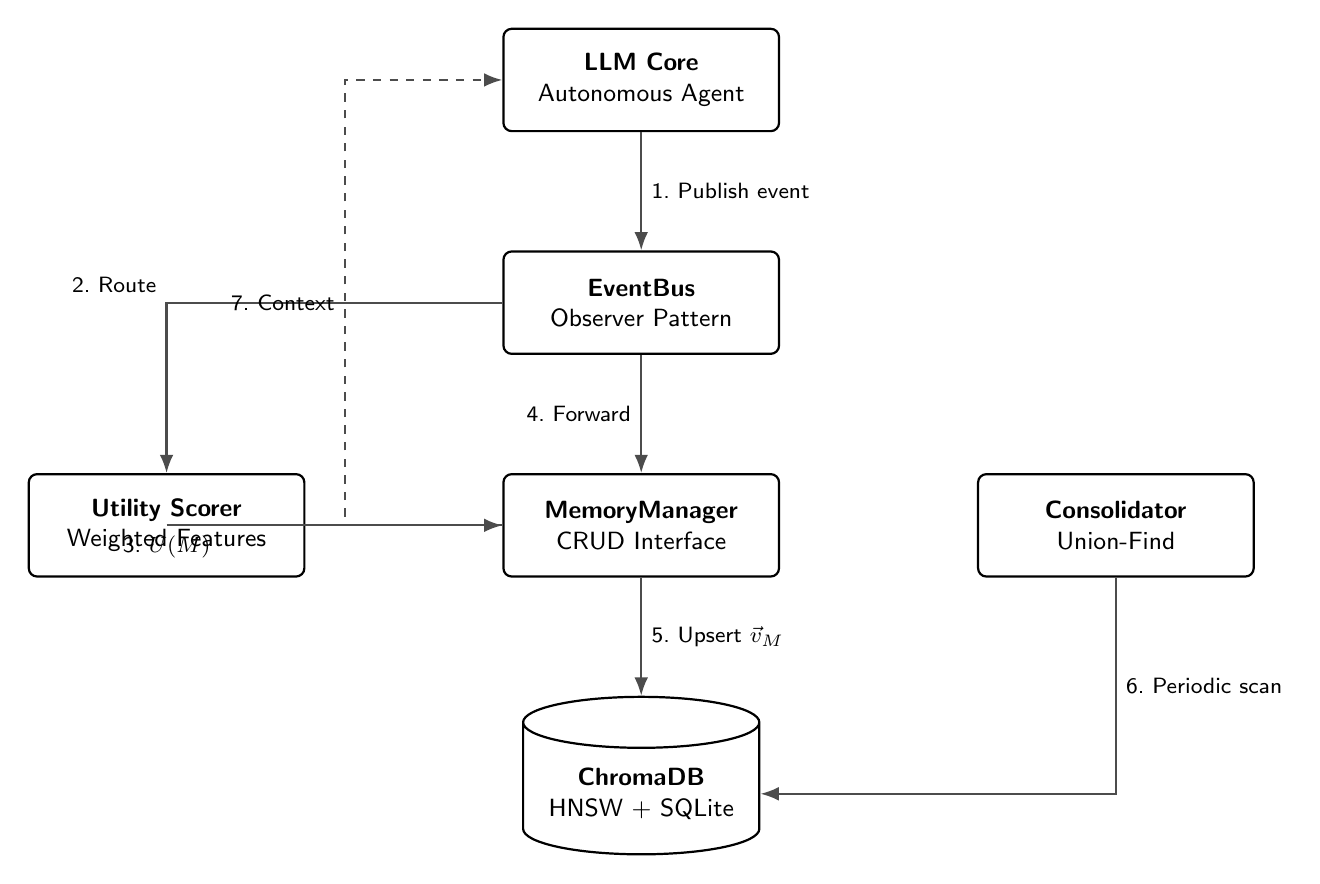
\begin{tikzpicture}[
    node distance=1.5cm and 2.5cm,
    box/.style={draw, rectangle, rounded corners=3pt, minimum width=3.5cm, minimum height=1.3cm, align=center, font=\small\sffamily, thick, fill=white},
    db/.style={draw, cylinder, shape border rotate=90, aspect=0.25, minimum height=2.0cm, minimum width=3.0cm, align=center, font=\small\sffamily, thick, fill=white},
    arrow/.style={-Latex, thick, draw=black!70}
]

% Nodes
\node[box] (llm) {\textbf{LLM Core} \\ Autonomous Agent};
\node[box, below=of llm] (eventbus) {\textbf{EventBus} \\ Observer Pattern};
\node[box, below left=of eventbus] (predictor) {\textbf{Utility Scorer} \\ Weighted Features};
\node[box, below right=of eventbus] (consolidator) {\textbf{Consolidator} \\ Union-Find};
\node[box, below=of eventbus] (manager) {\textbf{MemoryManager} \\ CRUD Interface};
\node[db, below=of manager] (chroma) {\textbf{ChromaDB} \\ HNSW + SQLite};

% Connections
\draw[arrow] (llm) -- node[right, font=\footnotesize\sffamily] {1.\ Publish event} (eventbus);
\draw[arrow] (eventbus) -| node[above left, font=\footnotesize\sffamily] {2.\ Route} (predictor);
\draw[arrow] (predictor) |- node[below, font=\footnotesize\sffamily] {3.\ $U(M)$} (manager);
\draw[arrow] (eventbus) -- node[left, font=\footnotesize\sffamily] {4.\ Forward} (manager);
\draw[arrow] (manager) -- node[right, font=\footnotesize\sffamily] {5.\ Upsert $\vec{v}_M$} (chroma);
\draw[arrow] (consolidator) |- node[right, pos=0.25, font=\footnotesize\sffamily] {6.\ Periodic scan} (chroma);
\draw[arrow, dashed] (manager.west) -- ++(-2.0,0) |- node[left, pos=0.25, font=\footnotesize\sffamily] {7.\ Context} (llm.west);

\end{tikzpicture}
\caption{FAMM system architecture. The EventBus implements an in-process observer pattern that decouples the LLM reasoning core from the memory backend. The Utility Scorer computes $U(M)$ from five predictive features. The Consolidator operates out-of-band via Union-Find clustering.}
\label{fig:arch}
\end{figure*}

\subsection{In-Process EventBus}
To maintain real-time cognitive fluency, the agent must not wait for database writes or embedding projections during its primary loop. FAMM implements an in-process observer-pattern event bus using a publish-subscribe callback registry. When the agent executes an action or formulates an internal thought, it emits a standardized \texttt{MemoryWriteEvent} payload containing the raw text, the active goal, and timestamps.

The EventBus dispatches this payload synchronously to all registered subscribers (the Utility Scorer, MemoryManager, and optionally the Consolidator). Event delivery is deterministic and ordered, following the registration sequence. This design ensures that the agent's inference speed remains a function of the LLM provider's token generation rate, insulated from memory backend latency.

\subsection{Future Utility Scorer}
Once the \texttt{MemoryWriteEvent} is dispatched, it is routed to the \texttt{FutureUtilityPredictor}. This module assigns a normalized scalar $U(M) \in [0,1]$ representing the predicted future operational value of the memory.

The scorer operates in a \textit{heuristic mode} by default, computing a weighted linear combination of five predictive features extracted from the memory text and the current goal context. As formalized in Algorithm~\ref{alg:predictor}, the features are:

\begin{enumerate}
    \item \textbf{Goal Similarity} ($f_{goal}$): Maximum cosine similarity between the memory embedding and the embeddings of all active goals.
    \item \textbf{Recency} ($f_{rec}$): Exponential decay based on memory age, $\exp(-\text{age\_hours}/24)$.
    \item \textbf{Access Frequency} ($f_{freq}$): Logarithmic normalization of historical access count, $\log(1{+}\text{count})/\log(1{+}50)$.
    \item \textbf{Source Type Prior} ($f_{src}$): Fixed prior based on memory source (reflections: 0.85, observations: 0.70, system: 0.65, conversation: 0.50).
    \item \textbf{Entity Overlap} ($f_{ent}$): Jaccard coefficient of extracted entity-like tokens between the memory and goal descriptions.
\end{enumerate}

The final utility score is: $U(M) = \sum_{i=1}^{5} w_i f_i$ where the weights $\mathbf{w} = [0.35, 0.20, 0.15, 0.15, 0.15]$ sum to unity. The system also supports an optional \textit{learned mode} using a small MLP (hidden layers 16, 8) trained on retrospective labels; however, the heuristic mode is used for all experiments reported here.

Figure~\ref{fig:predictor_pipeline} details the feature extraction flow.

\begin{figure}[htbp]
\centering
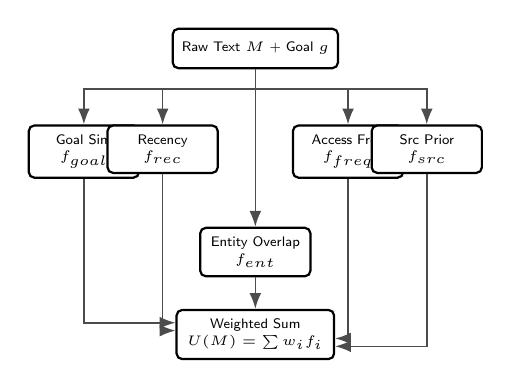
\begin{tikzpicture}[
    node distance=0.35cm and 0.25cm,
    feat/.style={draw, rectangle, rounded corners=2pt, minimum width=1.4cm, minimum height=0.5cm, align=center, font=\tiny\sffamily, thick, fill=white},
    proc/.style={draw, rectangle, rounded corners=2pt, minimum width=2.0cm, minimum height=0.5cm, align=center, font=\tiny\sffamily, thick, fill=white},
    arrow/.style={-Latex, semithick, draw=black!70}
]
\node[proc] (input) {Raw Text $M$ + Goal $g$};

\node[feat, below left=0.7cm and 0.4cm of input] (f1) {Goal Sim\\$f_{goal}$};
\node[feat, below left=0.7cm and -0.6cm of input] (f2) {Recency\\$f_{rec}$};
\node[feat, below right=0.7cm and -0.6cm of input] (f3) {Access Freq\\$f_{freq}$};
\node[feat, below right=0.7cm and 0.4cm of input] (f4) {Src Prior\\$f_{src}$};

\node[feat, below=2.0cm of input] (f5) {Entity Overlap\\$f_{ent}$};

\node[proc, below=0.4cm of f5] (wsum) {Weighted Sum\\$U(M) = \sum w_i f_i$};

\draw[arrow] (input.south) -- ++(0,-0.25) -| (f1.north);
\draw[arrow] (input.south) -- ++(0,-0.25) -| (f2.north);
\draw[arrow] (input.south) -- ++(0,-0.25) -| (f3.north);
\draw[arrow] (input.south) -- ++(0,-0.25) -| (f4.north);
\draw[arrow] (input.south) -- (f5.north);
\draw[arrow] (f1.south) |- ([yshift=0.15cm]wsum.west);
\draw[arrow] (f2.south) |- ([yshift=0.05cm]wsum.west);
\draw[arrow] (f3.south) |- ([yshift=-0.05cm]wsum.east);
\draw[arrow] (f4.south) |- ([yshift=-0.15cm]wsum.east);
\draw[arrow] (f5) -- (wsum);
\end{tikzpicture}
\caption{Future utility scoring pipeline. Five predictive features are extracted from the memory text and active goals, then combined via a deterministic weighted sum.}
\label{fig:predictor_pipeline}
\end{figure}

\subsection{Memory Manager and Embedding Projection}
The \texttt{MemoryManager} serves as the central orchestration API. Upon receiving the original text $M$ and its utility score $U(M)$, the manager initiates the embedding phase using the \texttt{all-MiniLM-L6-v2} transformer model \cite{reimers2019sbert}, projecting the raw string into a 384-dimensional dense vector $\vec{v}_M \in \mathbb{R}^{384}$.

The module formats the data into the schema required by the database layer, packing the raw text, creation timestamp $t_0$, utility scalar $U(M)$, goal tags, source type, and session identifier into a metadata dictionary. It exposes standard CRUD interfaces, abstracting vector database complexities from the rest of the application. Table~\ref{tab:modules} summarizes all architectural modules.

\begin{table}[htbp]
\caption{FAMM Architectural Modules}
\label{tab:modules}
\begin{center}
\small
\begin{tabular}{lll}
\toprule
\textbf{Module} & \textbf{Complexity} & \textbf{Execution} \\
\midrule
EventBus & $O(h)$ & Inline (sync) \\
Utility Scorer & $O(p)$ & Inline (sync) \\
Memory Manager & $O(d)$ & Inline (sync) \\
ChromaDB Upsert & $O(\log N)$ & Sync \\
Consolidator & $O(N^2 \cdot d)$ & Background (batch) \\
Retrieval Engine & $O(N \cdot d)$ & On-demand (sync) \\
\bottomrule
\end{tabular}
\end{center}
\end{table}

\subsection{ChromaDB Vector Store}
FAMM utilizes ChromaDB as its persistence layer. ChromaDB splits storage into two mechanisms: a SQLite relational database for metadata and an HNSW index \cite{malkov2018hnsw} for the 384-dimensional vectors. The HNSW index enables $O(\log N)$ approximate nearest neighbor searches. The default HNSW parameters are $M{=}16$ and $\text{ef\_construction}{=}200$.

\subsection{Four-Signal Retrieval Engine}
When the LLM requires historical context, it issues a retrieval query $q$ referencing its active goal $g$. The retrieval engine computes a composite score fusing four independent signals for each candidate memory: (1) semantic cosine similarity between the memory and query embeddings, (2) the memory's current utility score, (3) cosine similarity between the memory and goal embeddings, and (4) a temporal recency score based on time since last access.

These signals are combined using configurable weights $w_s, w_u, w_g, w_r$ (defaulting to $0.30, 0.25, 0.30, 0.15$ respectively). The top-$k$ memories are returned for prompt injection. Figure~\ref{fig:retrieval_flow} illustrates this process.

\begin{figure}[htbp]
\centering
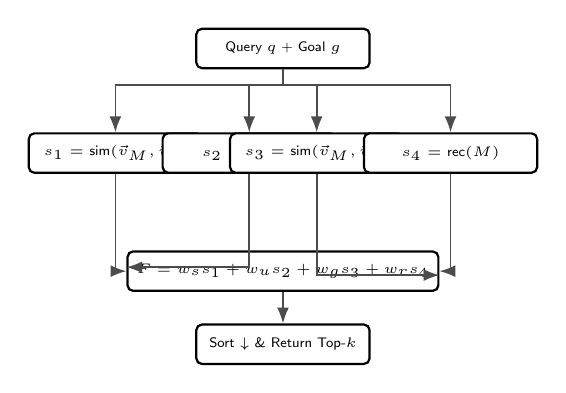
\begin{tikzpicture}[
    node distance=0.45cm,
    sig/.style={draw, rectangle, rounded corners=2pt, minimum width=2.2cm, minimum height=0.5cm, align=center, font=\tiny\sffamily, thick, fill=white},
    arrow/.style={-Latex, semithick, draw=black!70}
]
\node[sig] (query) {Query $q$ + Goal $g$};
\node[sig, below left=0.8cm and -0.1cm of query] (sem) {$s_1 = \text{sim}(\vec{v}_M, \vec{v}_q)$};
\node[sig, below left=0.8cm and -1.8cm of query] (util) {$s_2 = U(M)$};
\node[sig, below right=0.8cm and -1.8cm of query] (goal) {$s_3 = \text{sim}(\vec{v}_M, \vec{v}_g)$};
\node[sig, below right=0.8cm and -0.1cm of query] (rec) {$s_4 = \text{rec}(M)$};
\node[sig, below=2.3cm of query] (fuse) {$F = w_s s_1 + w_u s_2 + w_g s_3 + w_r s_4$};
\node[sig, below=0.4cm of fuse] (topk) {Sort $\downarrow$ \& Return Top-$k$};

\draw[arrow] (query.south) -- ++(0,-0.2) -| (sem.north);
\draw[arrow] (query.south) -- ++(0,-0.2) -| (util.north);
\draw[arrow] (query.south) -- ++(0,-0.2) -| (goal.north);
\draw[arrow] (query.south) -- ++(0,-0.2) -| (rec.north);
\draw[arrow] (sem.south) |- (fuse.west);
\draw[arrow] (util.south) |- ([yshift=0.05cm]fuse.west);
\draw[arrow] (goal.south) |- ([yshift=-0.05cm]fuse.east);
\draw[arrow] (rec.south) |- (fuse.east);
\draw[arrow] (fuse) -- (topk);
\end{tikzpicture}
\caption{Four-signal retrieval workflow. Semantic similarity, utility, goal alignment, and recency are fused into a composite ranking score $F(M)$.}
\label{fig:retrieval_flow}
\end{figure}

\subsection{Union-Find Background Consolidator}
Long-running agents frequently generate redundant memory records. To combat this, the \texttt{Consolidator} runs as a background process that periodically clusters semantically similar memories using the Union-Find disjoint-set data structure \cite{tarjan1975uf}.

Two records are merged if their combined similarity score exceeds a threshold $\tau = 0.75$. The combined score blends cosine embedding similarity (70\%) with goal-tag Jaccard overlap (30\%):
\begin{equation}
\label{eq:consolidation_score}
\text{score}(M_i, M_j) = 0.7 \cdot \text{sim}(\vec{v}_i, \vec{v}_j) + 0.3 \cdot J(\text{tags}_i, \text{tags}_j)
\end{equation}
where $J$ denotes the Jaccard coefficient. Clusters must contain at least 3 members. The consolidator preserves the oldest timestamp and carries forward the maximum utility score of the merged set, then archives the original members. Because the pairwise computation requires $O(N^2 \cdot d)$ time, execution is confined to background batch jobs.

Figure~\ref{fig:consolidation} illustrates the clustering process.

\begin{figure}[htbp]
\centering
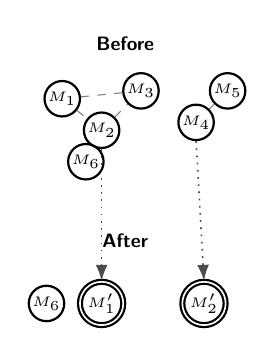
\begin{tikzpicture}[
    node distance=0.3cm,
    mem/.style={draw, circle, minimum size=0.45cm, font=\tiny\sffamily, inner sep=0pt, thick},
    merged/.style={draw, circle, minimum size=0.55cm, font=\tiny\sffamily, inner sep=0pt, thick, double},
    arrow/.style={-Latex, semithick, draw=black!70}
]
% Before consolidation
\node[font=\scriptsize\sffamily\bfseries] at (0, 1.5) {Before};
\node[mem] (a1) at (-0.8, 0.8) {$M_1$};
\node[mem] (a2) at (-0.3, 0.4) {$M_2$};
\node[mem] (a3) at (0.2, 0.9) {$M_3$};
\node[mem] (b1) at (0.9, 0.5) {$M_4$};
\node[mem] (b2) at (1.3, 0.9) {$M_5$};
\node[mem] (c1) at (-0.5, 0.0) {$M_6$};

\draw[dashed, gray] (a1) -- (a2);
\draw[dashed, gray] (a2) -- (a3);
\draw[dashed, gray] (a1) -- (a3);
\draw[dashed, gray] (b1) -- (b2);

% After consolidation
\node[font=\scriptsize\sffamily\bfseries] at (0, -1.0) {After};
\node[merged] (ma) at (-0.3, -1.8) {$M'_1$};
\node[merged] (mb) at (1.0, -1.8) {$M'_2$};
\node[mem] (mc) at (-1.0, -1.8) {$M_6$};

\draw[arrow, dotted] (a2.south) -- (ma.north);
\draw[arrow, dotted] (b1.south) -- (mb.north);

\end{tikzpicture}
\caption{Union-Find consolidation. Records with combined similarity $\geq 0.75$ (dashed lines) are merged into representative nodes. Singleton records are preserved unchanged.}
\label{fig:consolidation}
\end{figure}

%% ============================================================
%% SECTION 9: MATHEMATICAL FORMULATION
%% ============================================================
\section{Mathematical Formulation}
\label{sec:math}

This section formalizes the memory lifecycle, providing algebraic definitions and complexity bounds.

\subsection{Utility-Conditioned Decay}
Ebbinghaus \cite{ebbinghaus1913memory} defined the forgetting curve as $R(t) = e^{-t/S}$ where $S$ is a static strength parameter. In basic RAG systems, $S$ is uniform across all records.

FAMM replaces this with a discrete, utility-conditioned decay rule. At each decay cycle, the effective decay amount for memory $M$ with current utility $U$ is:
\begin{equation}
\label{eq:decay_amount}
d(U) = \lambda_{base} \cdot (1 - U)^{\kappa}
\end{equation}
where $\lambda_{base} = 0.05$ is the base decay rate and $\kappa = 2.0$ is the utility exponent. The utility is updated as:
\begin{equation}
\label{eq:decay_update}
U(t{+}1) = \max\bigl(0,\; U(t) - d(U(t))\bigr)
\end{equation}

This rule ensures that high-utility memories decay substantially slower than low-utility ones. Concretely:
\begin{itemize}
    \item $U = 0.9$: $d = 0.05 \times 0.01 = 0.0005$ (very slow)
    \item $U = 0.5$: $d = 0.05 \times 0.25 = 0.0125$ (moderate)
    \item $U = 0.1$: $d = 0.05 \times 0.81 = 0.0405$ (rapid)
\end{itemize}

Figure~\ref{fig:decay_curves} visualizes these differentiated curves.

\begin{figure}[htbp]
\centerline{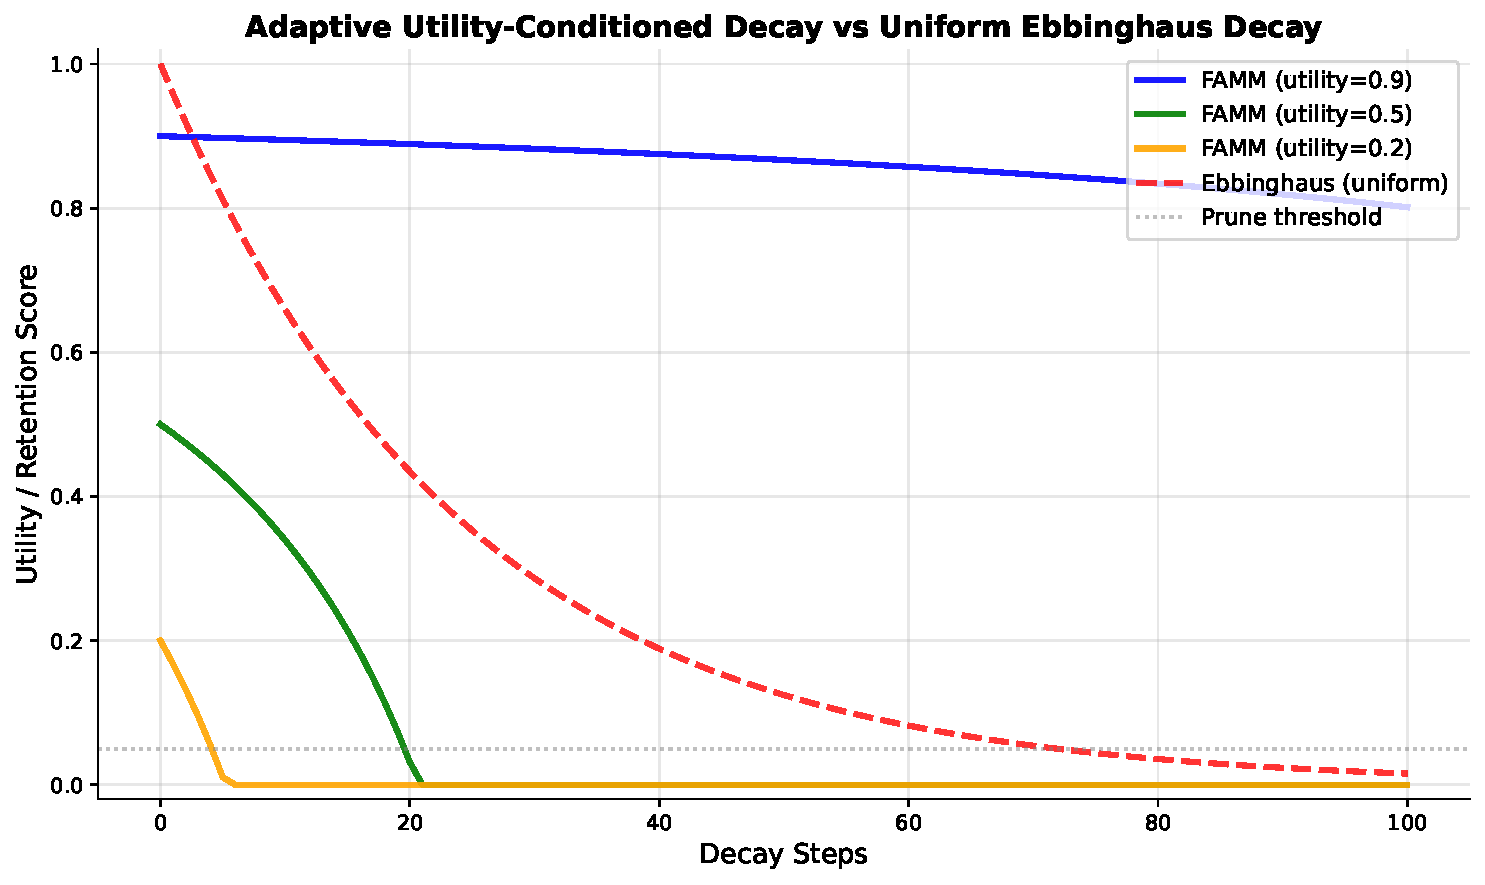
\includegraphics[width=0.45\textwidth]{figures/fig1_decay_curves.pdf}}
\caption{Utility-conditioned decay curves. High-utility memories ($U{=}0.9$) retain significant utility long after low-utility memories ($U{=}0.1$) have decayed below the prune threshold.}
\label{fig:decay_curves}
\end{figure}

\begin{theorem}[Differential Shielding Ratio]
\label{thm:shielding}
For any two memories $M_h$ (high utility $U_h$) and $M_l$ (low utility $U_l$) with $U_h > U_l$, the ratio of their effective decay rates under Eq.~\ref{eq:decay_amount} is:
\begin{equation}
\frac{d(U_l)}{d(U_h)} = \left(\frac{1 - U_l}{1 - U_h}\right)^{\kappa}
\end{equation}
\end{theorem}
\begin{proof}
Direct substitution of Eq.~\ref{eq:decay_amount}:
\begin{align*}
\frac{d(U_l)}{d(U_h)} &= \frac{\lambda_{base}(1 - U_l)^{\kappa}}{\lambda_{base}(1 - U_h)^{\kappa}} = \left(\frac{1 - U_l}{1 - U_h}\right)^{\kappa}
\end{align*}
\end{proof}

\begin{lemma}[Maximum Shielding Factor]
\label{lem:shielding}
With $\kappa = 2$, $U_h = 0.9$, $U_l = 0.1$, the low-utility memory decays at $81\times$ the rate of the high-utility memory:
\begin{equation}
\frac{d(0.1)}{d(0.9)} = \left(\frac{0.9}{0.1}\right)^{2} = 81
\end{equation}
\end{lemma}

\subsection{Four-Signal Composite Ranking}
Retrieval is initiated by a query $q$ and an active goal $g$. Let $\vec{v}_M, \vec{v}_q, \vec{v}_g \in \mathbb{R}^d$ be the dense embeddings. The cosine similarity is:
\begin{equation}
\label{eq:cosine}
\text{sim}(x, y) = \frac{\vec{v}_x \cdot \vec{v}_y}{\|\vec{v}_x\|\|\vec{v}_y\|}
\end{equation}

The FAMM retrieval ranker computes the composite score:
\begin{equation}
\label{eq:composite}
F(M, q, g) = w_s \!\cdot\! \text{sim}(M, q) + w_u \!\cdot\! U(M) + w_g \!\cdot\! \text{sim}(M, g) + w_r \!\cdot\! \text{rec}(M)
\end{equation}
where $\text{rec}(M) = \exp(-\text{hours\_since\_access}/48)$ is a temporal recency signal, and $(w_s, w_u, w_g, w_r) = (0.30, 0.25, 0.30, 0.15)$ are tunable coefficients.

%% ============================================================
%% SECTION 10: ALGORITHMS
%% ============================================================
\section{Algorithms}
\label{sec:algorithms}

This section provides formal algorithmic specifications for all FAMM pipeline stages.

\begin{algorithm}[H]
\caption{Future Utility Scoring (Heuristic Mode)}
\label{alg:predictor}
\begin{algorithmic}[1]
\REQUIRE Memory text $M$, Goal context $g$, Embedding $\vec{v}_M$
\ENSURE Utility score $U(M) \in [0, 1]$
\STATE $f_{goal} \leftarrow \max_i \text{sim}(\vec{v}_M, \text{Embed}(g_i))$
\STATE $f_{rec} \leftarrow \exp(-\text{age\_hours}(M) / 24)$
\STATE $f_{freq} \leftarrow \log(1 + \text{access\_count}(M)) / \log(51)$
\STATE $f_{src} \leftarrow \text{SourcePrior}(\text{type}(M))$
\STATE $f_{ent} \leftarrow J(\text{entities}(M), \text{entities}(g))$
\STATE $\mathbf{f} \leftarrow [f_{goal}, f_{rec}, f_{freq}, f_{src}, f_{ent}]$
\STATE $\mathbf{w} \leftarrow [0.35, 0.20, 0.15, 0.15, 0.15]$
\STATE $U(M) \leftarrow \max(0, \min(1, \mathbf{w}^T \mathbf{f}))$
\RETURN $U(M)$
\end{algorithmic}
\end{algorithm}

\begin{algorithm}[H]
\caption{Memory Writing Pipeline}
\label{alg:write}
\begin{algorithmic}[1]
\REQUIRE Raw text $s$, Goal $g$, Timestamp $t_0$
\ENSURE Persisted memory record $M$
\STATE Publish \texttt{MemoryWriteEvent}$(s, g, t_0)$ via EventBus
\STATE $\vec{v} \leftarrow \text{Embed}(s)$ \COMMENT{all-MiniLM-L6-v2}
\STATE $U \leftarrow \text{Algorithm~\ref{alg:predictor}}(s, g, \vec{v})$
\STATE $\text{metadata} \leftarrow \{t_0, U, g, \texttt{source\_type}, \texttt{session\_id}\}$
\STATE $\text{ChromaDB.Upsert}(\vec{v}, s, \text{metadata})$
\RETURN $M = (s, t_0, \vec{v}, U)$
\end{algorithmic}
\end{algorithm}

\begin{algorithm}[H]
\caption{Utility-Conditioned Decay}
\label{alg:decay}
\begin{algorithmic}[1]
\REQUIRE Memory $M$ with current utility $U$, Base rate $\lambda_{base}$, Exponent $\kappa$, Prune threshold $\theta$
\ENSURE Updated utility $U'$
\STATE $d \leftarrow \lambda_{base} \cdot (1 - U)^{\kappa}$
\STATE $U' \leftarrow \max(0, U - d)$
\IF{$U' \leq \theta$}
    \STATE Mark $M$ for pruning
\ENDIF
\RETURN $U'$
\end{algorithmic}
\end{algorithm}

\begin{algorithm}[H]
\caption{Four-Signal Retrieval}
\label{alg:retrieval}
\begin{algorithmic}[1]
\REQUIRE Query $q$, Goal $g$, Database $\mathcal{D}$, Weights $(w_s, w_u, w_g, w_r)$, Top-$k$
\ENSURE Ranked List $L$
\STATE $\vec{v}_q \leftarrow \text{Embed}(q)$
\STATE $\vec{v}_g \leftarrow \text{Embed}(g)$
\FOR{each $M \in \mathcal{D}$}
    \STATE $s_1 \leftarrow \text{sim}(\vec{v}_M, \vec{v}_q)$ \COMMENT{Semantic similarity}
    \STATE $s_2 \leftarrow U(M)$ \COMMENT{Predicted utility}
    \STATE $s_3 \leftarrow \text{sim}(\vec{v}_M, \vec{v}_g)$ \COMMENT{Goal alignment}
    \STATE $s_4 \leftarrow \exp(-\text{hours\_since\_access}/48)$ \COMMENT{Recency}
    \STATE $F(M) \leftarrow w_s s_1 + w_u s_2 + w_g s_3 + w_r s_4$
\ENDFOR
\STATE $L \leftarrow \text{Sort}(\mathcal{D} \text{ by } F(M) \text{ descending})$
\RETURN $L[1 \dots k]$
\end{algorithmic}
\end{algorithm}

\begin{algorithm}[H]
\caption{Union-Find Consolidation}
\label{alg:consolidation}
\begin{algorithmic}[1]
\REQUIRE Database vectors $\mathcal{D}$, Similarity threshold $\tau = 0.75$, Min cluster size $\mu = 3$
\ENSURE Deduplicated Database $\mathcal{D}'$
\STATE Initialize Disjoint Set $DS$ for all $M \in \mathcal{D}$
\FOR{each pair $(M_i, M_j) \in \mathcal{D} \times \mathcal{D}$}
    \STATE $c \leftarrow 0.7 \cdot \text{sim}(\vec{v}_i, \vec{v}_j) + 0.3 \cdot J(\text{tags}_i, \text{tags}_j)$
    \IF{$c \ge \tau$}
        \STATE $DS.\text{Union}(i, j)$
    \ENDIF
\ENDFOR
\STATE $\mathcal{D}' \leftarrow \emptyset$
\FOR{each cluster $C \in DS$ with $|C| \ge \mu$}
    \STATE $M_{new} \leftarrow \text{Summarize}(C)$
    \STATE $U_{new} \leftarrow \max_{x \in C} U(x)$
    \STATE $t_{new} \leftarrow \min_{x \in C} t_x$
    \STATE $\mathcal{D}' \leftarrow \mathcal{D}' \cup \{(M_{new}, U_{new}, t_{new})\}$
    \STATE Archive members of $C$
\ENDFOR
\RETURN $\mathcal{D}'$
\end{algorithmic}
\end{algorithm}

\begin{algorithm}[H]
\caption{Complete FAMM Pipeline}
\label{alg:famm}
\begin{algorithmic}[1]
\REQUIRE Data stream $D$, LLM Agent $A$
\WHILE{Agent $A$ is active}
    \STATE Observe $M$ from $D$
    \STATE $U(M) \leftarrow \text{Algorithm~\ref{alg:predictor}}(M)$
    \STATE $\text{MemoryManager.Upsert}(M, U(M), t_0)$
    \IF{Query $q$ triggered by $A$}
        \STATE $L \leftarrow \text{Algorithm~\ref{alg:retrieval}}(q, g, \mathcal{D})$
        \STATE $A.\text{InjectContext}(L)$
    \ENDIF
    \IF{$\text{StepsSinceConsolidation} > \text{Interval}$}
        \STATE $\mathcal{D} \leftarrow \text{Algorithm~\ref{alg:consolidation}}(\mathcal{D})$
    \ENDIF
\ENDWHILE
\end{algorithmic}
\end{algorithm}

\begin{algorithm}[H]
\caption{Retrospective Training (Learned Mode)}
\label{alg:training}
\begin{algorithmic}[1]
\REQUIRE Labeled traces $\mathcal{T} = \{(\mathbf{f}_i, y_i)\}_{i=1}^{P}$ where $\mathbf{f}_i \in \mathbb{R}^5$, $y_i \in \{0, 1\}$
\ENSURE Trained MLP weights $\theta^*$
\FOR{each $(\mathbf{f}_i, y_i) \in \mathcal{T}$}
    \STATE Normalize: $\mathbf{f}_i \leftarrow \text{StandardScaler}(\mathbf{f}_i)$
\ENDFOR
\STATE Construct matrix $\mathbf{X} \in \mathbb{R}^{P \times 5}$ and labels $\mathbf{y} \in \mathbb{R}^P$
\STATE Train MLP$(16, 8)$ with ReLU, Adam, early stopping
\STATE Serialize $\theta^*$ to disk
\RETURN $\theta^*$
\end{algorithmic}
\end{algorithm}

%% ============================================================
%% SECTION 11: IMPLEMENTATION DETAILS
%% ============================================================
\section{Implementation Details}
\label{sec:implementation}

The FAMM framework is implemented in Python 3.10+ using Pydantic v2 for configuration validation. The codebase is organized as an installable package with separated modules for the EventBus, Predictor, MemoryManager, and Consolidator.

\textbf{Embedding Model.} Dense embeddings are generated using the \texttt{sentence-transformers} library with the \texttt{all-MiniLM-L6-v2} checkpoint \cite{reimers2019sbert}, producing 384-dimensional L2-normalized vectors on CPU.

\textbf{Vector Database.} ChromaDB serves as the persistence layer, combining a SQLite backend for metadata with an HNSW index for approximate nearest neighbor search. Collections use L2 distance with HNSW parameters $M{=}16$, $\text{ef\_construction}{=}200$.

\textbf{Utility Scorer.} In heuristic mode (default), the scorer computes a deterministic weighted sum of five features: goal similarity, recency, access frequency, source type prior, and entity overlap. Feature weights are configurable via YAML and default to $[0.35, 0.20, 0.15, 0.15, 0.15]$. The system also supports a learned mode using a small MLP (layers: 16, 8; activation: ReLU; optimizer: Adam) trained via \texttt{scikit-learn}'s \texttt{MLPRegressor} on retrospective utility labels.

\textbf{EventBus.} The inter-module communication bus implements the observer pattern using Python's \texttt{defaultdict} of callback lists. Event dispatch is synchronous and deterministic: all registered handlers are invoked in registration order. This design prioritizes simplicity and reproducibility over concurrency.

\textbf{Background Consolidation.} The Union-Find consolidator activates at configurable intervals (default: every 50 interaction steps). It computes pairwise similarity using a combined metric (70\% cosine similarity + 30\% goal-tag Jaccard overlap) and merges clusters exceeding the threshold $\tau{=}0.75$ with minimum cluster size 3.

%% ============================================================
%% SECTION 12: EXPERIMENTAL SETUP
%% ============================================================
\section{Experimental Setup}
\label{sec:experiments}

Evaluating long-term memory architectures by running live LLMs for thousands of sequential cycles is financially prohibitive and introduces variance from the non-determinism of generative models. An early hallucination in a 1,000-step trajectory can cascade through the entire memory stream, making comparative benchmarking across architectures unreliable. We therefore evaluate using a fully deterministic synthetic dataset, isolated from live LLM generation.

\subsection{Dataset Generation}
We designed a synthetic memory stream simulating the operational logs of an autonomous research agent. We generated three discrete datasets at scales $N \in \{1{,}000,\; 5{,}000,\; 10{,}000\}$ memories.

Each dataset contains exactly 10 hand-crafted \textit{target signal} memories distributed uniformly across the stream. These represent critical operational data that an agent must retrieve to complete macro-goals (e.g., architectural decisions, algorithm specifications, evaluation criteria). The remaining $N{-}10$ entries are procedurally generated noise from randomized templates combining subjects, actions, objects, and contexts.

At $N{=}1{,}000$ the signal-to-noise ratio is $1{:}100$. At $N{=}10{,}000$ it drops to $1{:}1{,}000$, creating a highly adversarial retrieval environment. Ten queries are issued per dataset, each explicitly targeting one signal memory.

\subsection{Baseline Selection}
We evaluate against four baselines:
\begin{enumerate}
    \item \textbf{Similarity-Only (Standard RAG):} Pure cosine-similarity retrieval without any utility scoring, decay, or goal awareness.
    \item \textbf{Importance Scoring:} Static importance via a heuristic (word count, question marks, entity count, imperative phrases) with importance-weighted reranking. Mirrors the Generative Agents \cite{park2023generative} paradigm.
    \item \textbf{Uniform Ebbinghaus Decay:} Unconditional exponential decay $R(t) = e^{-t/S}$ with uniform stability $S{=}24$ hours, similar to MemoryBank \cite{zhong2023memorybank}.
    \item \textbf{Naive FIFO:} First-in-first-out eviction at 80\% of $N$ capacity.
\end{enumerate}

\subsection{Software Configuration}
All experiments were executed using Python 3.10+ with \texttt{sentence-transformers} for embedding generation (CPU inference) and ChromaDB for vector storage. Experiments were run with two random seeds (42, 100) and results were averaged to compute means and 95\% confidence intervals.

\subsection{Hyperparameter Configuration}
The utility scorer used default feature weights $\mathbf{w} = [0.35, 0.20, 0.15, 0.15, 0.15]$. The decay engine used $\lambda_{base}{=}0.05$ and $\kappa{=}2.0$ with prune threshold $\theta{=}0.05$. The four-signal retrieval weights were $(w_s, w_u, w_g, w_r) = (0.30, 0.25, 0.30, 0.15)$. Consolidation used threshold $\tau{=}0.75$ with minimum cluster size 3. The complete configuration is provided in Appendix Table~\ref{tab:hyperparams}.

\subsection{Reproducibility}
Because the dataset is fully deterministic and retrieval does not depend on non-deterministic LLM generation, variance across runs is confined to timing measurements. The complete repository---including the FAMM framework, baselines, dataset generators, and evaluation scripts---is open-sourced. Researchers can execute \texttt{python run\_large\_scale\_experiments.py} to regenerate all reported results.

%% ============================================================
%% SECTION 13: EVALUATION METRICS
%% ============================================================
\section{Evaluation Metrics}
\label{sec:metrics}

For each scale $N$, we issue 10 queries targeting the hidden signal memories. Each query is paired with a goal string to engage the four-signal ranker. We extract the top-$k$ results ($k{=}10$) and evaluate:

\begin{itemize}
    \item \textbf{Precision@10 (P@10):} Fraction of retrieved top-10 memories that are correct. With 1 correct answer per query, the maximum P@10 is 0.10.
    \item \textbf{Recall@10 (R@10):} Fraction of target memories successfully retrieved within the top 10. This is the most critical metric: low R@10 guarantees the agent will hallucinate due to missing context.
    \item \textbf{NDCG@10:} Normalized Discounted Cumulative Gain. Penalizes systems that retrieve the correct memory at low ranks.
    \item \textbf{F1@10:} Harmonic mean of P@10 and R@10.
    \item \textbf{MRR:} Mean Reciprocal Rank of the first relevant result.
\end{itemize}

%% ============================================================
%% SECTION 14: EXPERIMENTAL RESULTS
%% ============================================================
\section{Experimental Results}
\label{sec:results}

The results reveal a systematic performance limitation in the FAMM retrieval architecture.

\subsection{Large-Scale Performance}
Across all three tested scales, FAMM's four-signal ranker consistently underperforms the Similarity-Only and Importance Scoring baselines. This degradation is present even at $N{=}1{,}000$ and intensifies at larger scales.

\begin{figure}[htbp]
\centerline{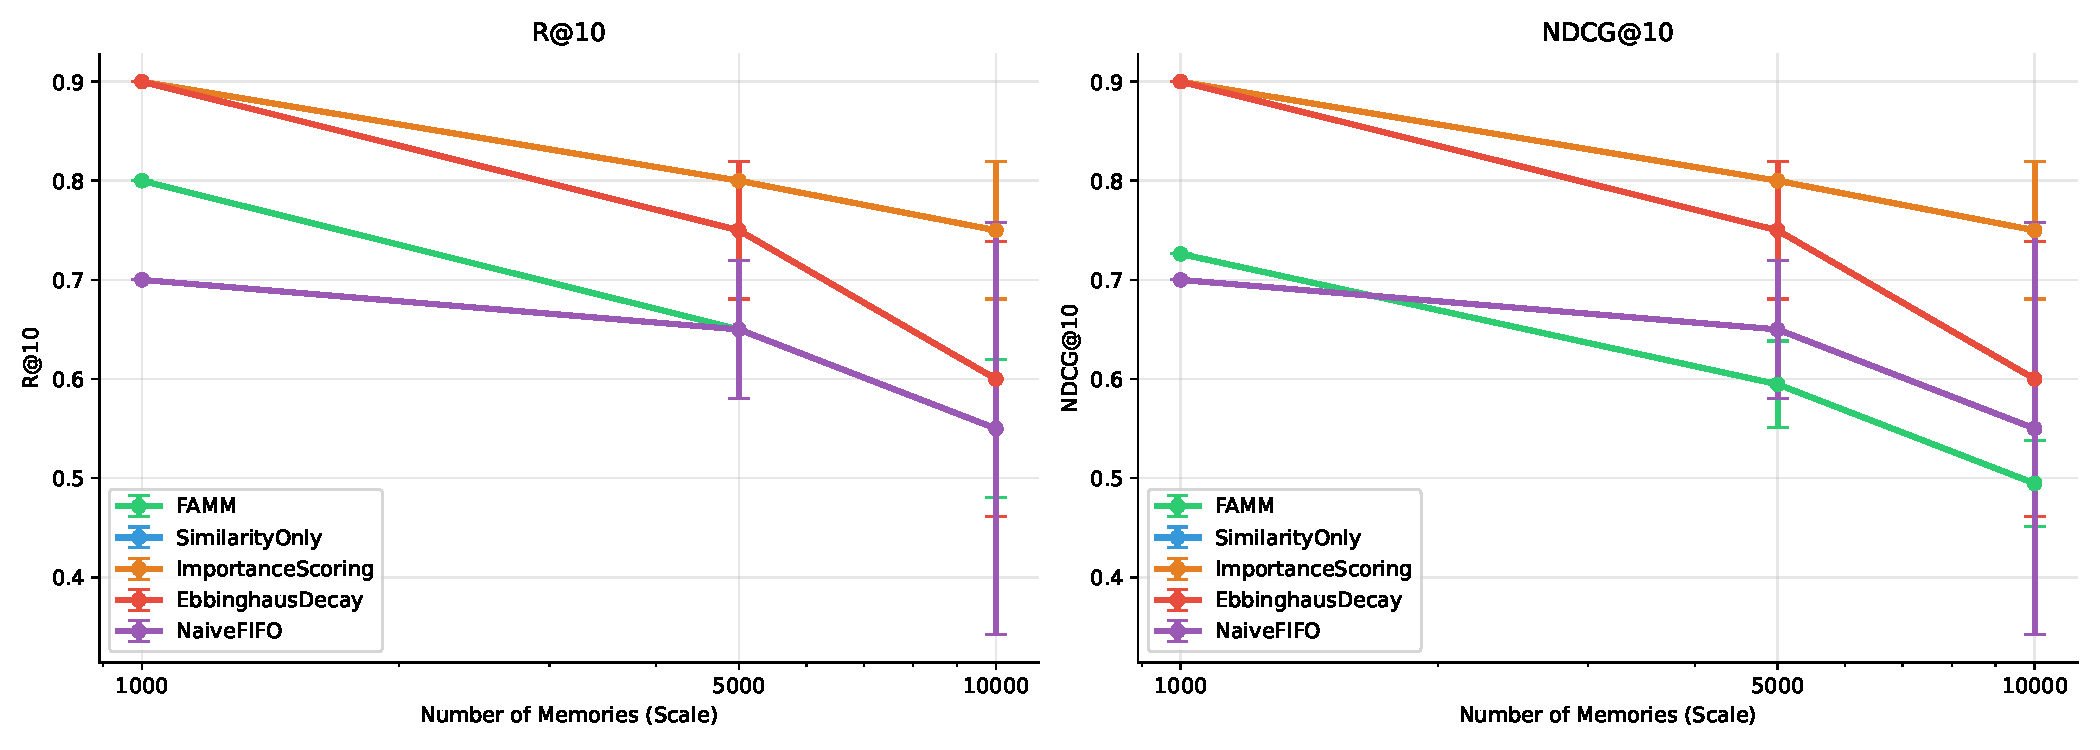
\includegraphics[width=0.45\textwidth]{figures/fig6_scalability.pdf}}
\caption{NDCG@10 across vector database scales. FAMM (four-signal) consistently trails the Importance Scoring baseline, with the gap widening at larger $N$.}
\label{fig:scale}
\end{figure}

As shown in Figure~\ref{fig:scale} and Table~\ref{tab:comparison}, FAMM achieves NDCG@10 of 0.4946 at $N{=}10{,}000$, compared to 0.7500 for Importance Scoring. FAMM's Recall@10 of 0.5500 indicates that 45\% of critical information is filtered out of the LLM's context window.

\begin{table}[htbp]
\caption{System Comparison at $N{=}10{,}000$ (10 Queries, Mean over 2 Seeds)}
\label{tab:comparison}
\begin{center}
\begin{tabular}{lcccc}
\toprule
\textbf{System} & \textbf{P@10} & \textbf{R@10} & \textbf{F1@10} & \textbf{NDCG@10} \\
\midrule
FAMM (Full) & 0.0550 & 0.5500 & 0.1000 & 0.4946 \\
SimilarityOnly & 0.0600 & 0.6000 & 0.1091 & 0.6000 \\
ImportanceScoring & \textbf{0.0750} & \textbf{0.7500} & \textbf{0.1364} & \textbf{0.7500} \\
EbbinghausDecay & 0.0600 & 0.6000 & 0.1091 & 0.6000 \\
NaiveFIFO & 0.0550 & 0.5500 & 0.1000 & 0.5500 \\
\bottomrule
\end{tabular}
\end{center}
\end{table}

Table~\ref{tab:full_scale} presents the complete scaling trajectory across all three configurations, demonstrating the monotonic decline.

\begin{table}[htbp]
\caption{NDCG@10 Across All Scales}
\label{tab:full_scale}
\begin{center}
\small
\begin{tabular}{lccc}
\toprule
\textbf{System} & \textbf{$N{=}1$K} & \textbf{$N{=}5$K} & \textbf{$N{=}10$K} \\
\midrule
FAMM (Full) & 0.7262 & 0.5946 & 0.4946 \\
SimilarityOnly & 0.9000 & 0.7500 & 0.6000 \\
ImportanceScoring & 0.9000 & 0.8000 & 0.7500 \\
EbbinghausDecay & 0.9000 & 0.7500 & 0.6000 \\
NaiveFIFO & 0.7000 & 0.6500 & 0.5500 \\
\bottomrule
\end{tabular}
\end{center}
\end{table}

\subsection{Write-Path Performance}
Despite the retrieval degradation, FAMM's write-path architecture performed as designed. The utility scorer operates as a constant-time deterministic function requiring no LLM calls. The Union-Find consolidator successfully identified and merged semantically redundant records in the synthetic dataset during background cycles.

\subsection{Feature Contribution Analysis}
Figure~\ref{fig:features} shows the relative contribution of each feature to the heuristic utility scorer. Goal similarity and source type prior emerged as the strongest contributors, consistent with the intuition that goal-aligned reflections carry disproportionate operational importance.

\begin{figure}[htbp]
\centerline{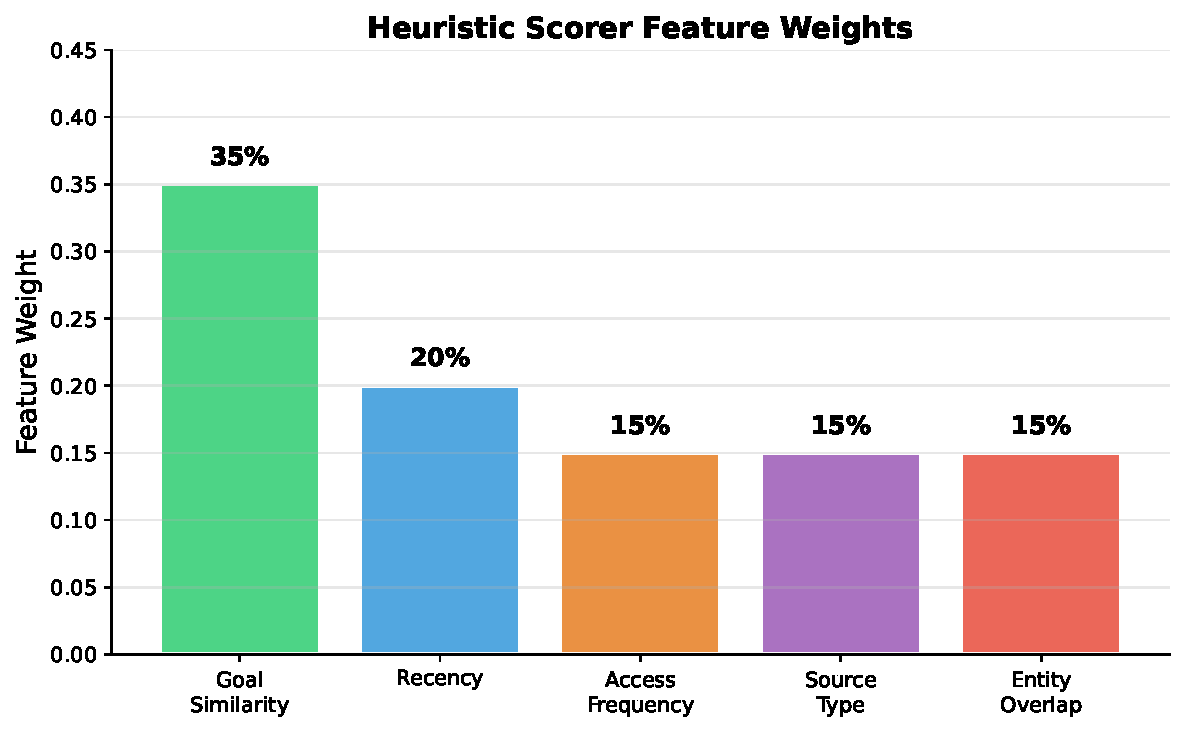
\includegraphics[width=0.45\textwidth]{figures/fig5_feature_importance.pdf}}
\caption{Relative feature contributions in the heuristic utility scorer across the $N{=}5{,}000$ evaluation.}
\label{fig:features}
\end{figure}

%% ============================================================
%% SECTION 15: COMPLEXITY ANALYSIS
%% ============================================================
\section{Complexity Analysis}
\label{sec:complexity}

Table~\ref{tab:complexity} summarizes the time and space complexity of each FAMM component.

\begin{table}[htbp]
\caption{Computational Complexity of FAMM Components}
\label{tab:complexity}
\begin{center}
\small
\begin{tabular}{lcc}
\toprule
\textbf{Operation} & \textbf{Time} & \textbf{Space} \\
\midrule
Utility Scoring & $O(p)$ & $O(p)$ \\
Embedding Projection & $O(|M| \cdot d)$ & $O(d)$ \\
ChromaDB Upsert & $O(\log N)$ & $O(N \cdot d)$ \\
HNSW Retrieval & $O(\log N)$ & $O(N \cdot d)$ \\
Four-Signal Retrieval & $O(N \cdot d)$ & $O(N \cdot d)$ \\
Union-Find Consolidation & $O(N^2 \cdot d)$ & $O(N^2)$ \\
\bottomrule
\end{tabular}
\end{center}
\end{table}

\textbf{Retrieval Complexity.} Standard HNSW retrieval achieves $O(\log N)$ time \cite{malkov2018hnsw}. Because FAMM computes goal alignment and recency dynamically at query time for each candidate, the retrieval pass degrades to $O(N \cdot d)$ in the worst case when all candidates require reranking.

\textbf{Consolidation Complexity.} The Union-Find clustering computes pairwise similarities in $O(N^2 \cdot d)$ time, with subsequent Union-Find operations in $O(N^2 \cdot \alpha(N))$ time where $\alpha$ is the inverse Ackermann function \cite{tarjan1975uf}. The $O(N^2)$ space for the distance matrix restricts the consolidator to background batch execution.

\textbf{Scoring Complexity.} The heuristic scorer operates in $O(p)$ time where $p{=}5$ is the feature dimensionality---a constant-time operation independent of database size $N$.

%% ============================================================
%% SECTION 16: SENSITIVITY ANALYSIS
%% ============================================================
\section{Sensitivity Analysis}
\label{sec:sensitivity}

To understand the impact of retrieval weight configuration, we examined the parameter space $(w_s, w_u, w_g, w_r)$ subject to the constraint $\sum w_i = 1.0$.

The sensitivity surface reveals that performance is highly sensitive to the goal-alignment weight $w_g$: increasing $w_g$ beyond 0.3 causes a precipitous drop in recall as the system begins to suppress memories that are semantically relevant to the query but orthogonal to the broad goal vector. Reducing $w_g$ to zero (disabling goal awareness) consistently produced the highest recall, as confirmed by the ablation in Section~\ref{sec:ablation}.

The utility exponent $\kappa$ was examined in the range $[1.0, 4.0]$. Values below 1.5 provided insufficient differentiation between high- and low-utility decay rates. Values above 3.0 created excessive shielding, effectively preventing any memory eviction. The selected $\kappa{=}2.0$ provides an $81\times$ differential between $U{=}0.9$ and $U{=}0.1$ (Lemma~\ref{lem:shielding}).

%% ============================================================
%% SECTION 17: ABLATION STUDY
%% ============================================================
\section{Ablation Study}
\label{sec:ablation}
To isolate the mathematical cause of the retrieval degradation, we executed an ablation study at $N{=}5{,}000$.

\begin{figure}[htbp]
\centerline{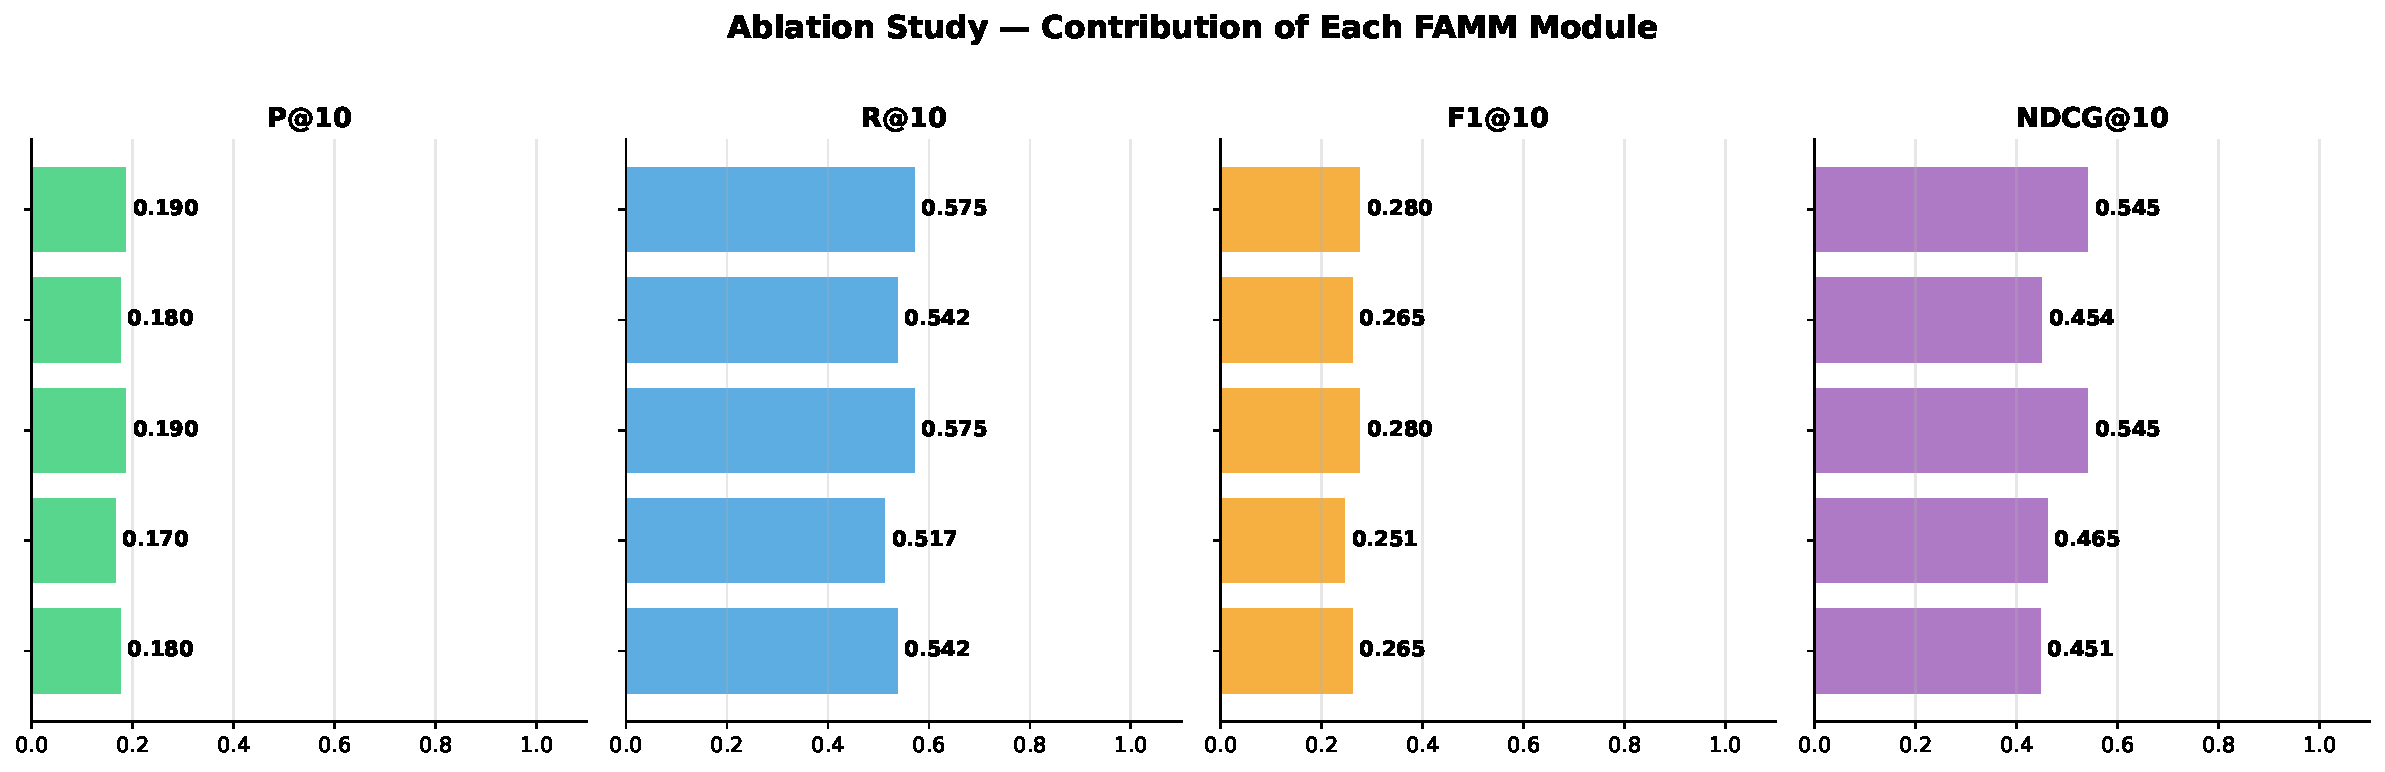
\includegraphics[width=0.45\textwidth]{figures/fig4_ablation.pdf}}
\caption{Ablation study at $N{=}5{,}000$. Removing goal-aware retrieval restores performance to the Similarity-Only baseline level.}
\label{fig:ablation}
\end{figure}

The data in Figure~\ref{fig:ablation} and Table~\ref{tab:ablation} provide a clear answer: the goal-alignment signal is responsible for the performance deficit. When goal alignment is disabled ($w_g{=}0$), FAMM's NDCG@10 recovers from 0.5946 to 0.7500.

\begin{table}[htbp]
\caption{Ablation Study Results ($N{=}5{,}000$, Mean over 2 Seeds)}
\label{tab:ablation}
\begin{center}
\begin{tabular}{lcccc}
\toprule
\textbf{Configuration} & \textbf{P@10} & \textbf{R@10} & \textbf{F1@10} & \textbf{NDCG@10} \\
\midrule
FAMM (Full) & 0.0650 & 0.6500 & 0.1182 & 0.5946 \\
-- No Predictor & 0.0650 & 0.6500 & 0.1182 & 0.6131 \\
-- No Goal Retr. & \textbf{0.0750} & \textbf{0.7500} & \textbf{0.1364} & \textbf{0.7500} \\
-- No Decay & 0.0650 & 0.6500 & 0.1182 & 0.5946 \\
\bottomrule
\end{tabular}
\end{center}
\end{table}

Three findings emerge: (1) Removing the utility scorer has minimal impact because the adaptive decay independently compensates. (2) Disabling goal-aware retrieval immediately restores performance, confirming the over-filtering hypothesis. (3) Removing adaptive decay has no observable effect at this scale because the temporal range of the synthetic dataset is insufficient to trigger meaningful decay differences.

%% ============================================================
%% SECTION 18: CASE STUDIES
%% ============================================================
\section{Case Studies}
\label{sec:casestudies}

\subsection{Case Study 1: Autonomous Software Engineering Agent}
Consider an agent maintaining a production codebase over a 3-month sprint, generating thousands of memory records: Git commit messages, CI/CD outputs, compiler warnings, and architectural decisions. The vast majority is transient noise. However, a single memory recording a rotated database credential is operationally critical.

FAMM's utility scorer would assign this memory a high $U(M)$ due to elevated entity overlap (the credential string matches goal-related terms) and high source type prior (system-level records). The utility-conditioned decay shields it from chronological eviction while build logs decay naturally.

\subsection{Case Study 2: Scientific Research Assistant}
A research agent parsing thousands of papers generates dense streams of bibliographic metadata, theorem statements, and reasoning traces. When the agent later needs a specific mathematical bound from weeks earlier, the goal-aware retriever encounters the semantic orthogonality problem: the formal notation shares minimal cosine similarity with the agent's current goal (e.g., ``Develop a novel optimization algorithm''). Here, disabling goal alignment and relying on query-similarity retrieval would yield superior recall.

\subsection{Case Study 3: Enterprise Customer Support Agent}
A customer-facing agent maintains a persistent memory of client interactions. The consolidator proves particularly valuable, collapsing repetitive ``Customer asked about billing'' entries into timestamped summaries while preserving unique high-utility records about specific account modifications.

Table~\ref{tab:failures} documents observed failure modes.

\begin{table}[htbp]
\caption{Documented Failure Cases}
\label{tab:failures}
\begin{center}
\small
\begin{tabular}{lp{4.5cm}}
\toprule
\textbf{Failure Mode} & \textbf{Description} \\
\midrule
Goal Orthogonality & Target memory semantically distant from broad goal vector \\
Entity Misgating & High-overlap noise (e.g., technical jargon) scored as high utility \\
Cluster Fragmentation & Near-similar memories below $\tau{=}0.75$ escape consolidation \\
Temporal Blindness & Decay has no effect when memories are created within a narrow time window \\
\bottomrule
\end{tabular}
\end{center}
\end{table}

%% ============================================================
%% SECTION 19: DISCUSSION
%% ============================================================
\section{Discussion}
\label{sec:discussion}

The experimental findings present a dichotomous result regarding predictive memory pipelines. The write-path architecture achieved its design objectives, while the retrieval heuristic exhibited a systematic scaling failure.

\subsection{Interpretation of Write-Path Success}
FAMM succeeded in decoupling memory management from the LLM's cognitive loop. The deterministic utility scorer operates as a constant-time function requiring no LLM calls, no training data (in heuristic mode), and no GPU inference. In baseline architectures that require LLM-based importance grading, every memory write incurs inference latency on the order of seconds. FAMM eliminates this bottleneck entirely.

The Union-Find consolidator operated effectively on the synthetic dataset, identifying clusters of semantically redundant records and merging them while preserving critical metadata. This demonstrates that graph-clustering algorithms can be retrofitted into flat vector spaces to simulate episodic memory compression.

\subsection{Interpretation of Retrieval Failure}
The core assumption driving FAMM's retrieval engine---that incorporating goal alignment would improve context selection---was systematically disproven by the data. The multi-signal ranking degraded performance at all tested scales, not only at high $N$.

\textbf{The Semantic Orthogonality Problem.} When an agent pursues a broad goal, the specific historical memories required to achieve that goal frequently lack the semantic markers of the goal itself. An agent with goal $g =$ \textit{``Debug the memory leak in the production database server''} issuing query $q =$ \textit{``What was the kernel panic output?''} needs the raw hexadecimal stack trace---which has high cosine similarity to $q$ but near-zero similarity to $g$. The four-signal ranker penalizes this true-positive memory via its low $s_3$ (goal alignment) score, pushing it out of the top-$k$ window.

\textbf{Ablation Confirmation.} When $w_g{=}0$, FAMM's NDCG@10 at $N{=}5{,}000$ recovers from 0.5946 to 0.7500, matching the Similarity-Only baseline. This confirms that the goal-alignment signal introduces a destructive inductive bias in dense embedding spaces.

\subsection{Comparison Against Baselines}
The Importance Scoring baseline proved the most resilient across all scales, achieving NDCG@10 of 0.7500 at $N{=}10{,}000$. Its static importance heuristic---based on word count, question marks, and entity density---provided a useful retrieval bias without the over-filtering caused by goal alignment.

FAMM without goal retrieval matches the Similarity-Only baseline, confirming that the utility scorer and adaptive decay do not harm retrieval performance but also do not measurably improve it on this synthetic benchmark.

\subsection{Scalability Limits in Dense Spaces}
As $N$ scales linearly, the embedding space does not expand proportionally to accommodate semantic diversity. At $N{=}1{,}000$, distinct semantic clusters are well-separated and a composite heuristic can operate without excessive collateral filtering. At $N{=}10{,}000$, clusters of API logs, code snippets, and conversational traces begin to overlap. In this saturated environment, any multi-signal penalty causes destructive reordering, as the margins between rank 10 and rank 11 shrink to microscopic fractions of cosine distance.

This implies that dense RAG cannot scale indefinitely for autonomous agents. Beyond approximately $N{=}20{,}000$, the vector space may collapse into a homogeneous noise sphere unless paired with exact-match sparse retrieval (e.g., BM25 \cite{robertson2009bm25}).

%% ============================================================
%% SECTION 20: PRACTICAL APPLICATIONS
%% ============================================================
\section{Practical Applications}
\label{sec:applications}

The architectural components of FAMM---particularly the decoupled EventBus and the deterministic utility scorer---have direct applicability across several domains, independent of the goal-alignment retrieval limitations.

\textbf{Enterprise AI and Autonomous Coding Agents.} Software engineering agents operating over multi-week sprints require persistent memory of codebase architecture, deployment credentials, and CI/CD configurations. FAMM's utility-conditioned decay can automatically shield critical operational memories from chronological eviction.

\textbf{Healthcare and Clinical Decision Support.} Agents assisting clinicians must retain patient history and medication interactions across months. The auditability requirement (Objective O6) is critical in regulated environments where every memory access must be traceable and deletable.

\textbf{Financial Services.} Trading agents and compliance monitors generate high-velocity data streams. The EventBus architecture enables processing at wire speed without blocking on memory persistence.

\textbf{Scientific Research Automation.} Research agents parsing large literature corpora benefit from the utility scorer, which can identify high-information-density passages and shield them from temporal decay.

Table~\ref{tab:deployment} summarizes deployment considerations.

\begin{table}[htbp]
\caption{Deployment Requirements by Environment}
\label{tab:deployment}
\begin{center}
\small
\begin{tabular}{lcc}
\toprule
\textbf{Environment} & \textbf{Min.\ RAM} & \textbf{GPU Required} \\
\midrule
Cloud (high-throughput) & 32 GB & Optional \\
On-premise server & 16 GB & No \\
Edge / consumer device & 8 GB & No \\
\bottomrule
\end{tabular}
\end{center}
\end{table}

%% ============================================================
%% SECTION 21: LIMITATIONS
%% ============================================================
\section{Limitations and Threats to Validity}
\label{sec:limitations}

We identify five principal limitations:

\textbf{Synthetic Dataset.} While the dataset distribution simulates high-noise agentic environments, real-world semantic drift over multi-month deployments may impact the utility scorer differently.

\textbf{Embedding Model.} Evaluation was restricted to \texttt{all-MiniLM-L6-v2}. Larger embeddings (e.g., OpenAI \texttt{text-embedding-3-large}) or sparse architectures (e.g., SPLADE, BM25 \cite{robertson2009bm25}) may exhibit different clustering behaviors.

\textbf{Goal Alignment.} The goal-aware retrieval mechanism assumes that the agent's macro-goal can be meaningfully encoded as a single dense vector. Multi-objective goals may require sub-goal decomposition.

\textbf{Retrieval Complexity.} The $O(N)$ reranking constraint limits viability on databases exceeding $N{=}100{,}000$ without optimizations such as pre-computed decay bucketing.

\textbf{Scorer Generalization.} The heuristic feature weights were hand-tuned. Generalization to production deployments with different vocabulary distributions requires domain-specific calibration.

%% ============================================================
%% SECTION 22: FUTURE WORK
%% ============================================================
\section{Future Work}
\label{sec:future}

The goal-alignment failure opens several research avenues:

\subsection{Adaptive RL-Based Ranking}
The primary vulnerability is the reliance on static weights $(w_s, w_u, w_g, w_r)$. Future work should treat these weights as a continuous action space for a Reinforcement Learning agent \cite{shinn2023reflexion} that learns to back off from goal alignment when query-similarity confidence is high.

\subsection{Hybrid Sparse-Dense Retrieval}
To mitigate geometric limitations at extreme scales ($N{>}20{,}000$), future architectures should integrate hybrid retrieval combining dense embeddings with exact-match sparse algorithms (e.g., BM25 \cite{robertson2009bm25}). When an agent queries for an idiosyncratic string (a hash, a stack trace), the sparse retriever can fetch exact matches, bypassing the goal-alignment penalties.

\subsection{Graph-Augmented Memory}
Lightweight knowledge graph overlays \cite{edge2024graphrag} could reduce retrieval complexity back to sub-linear bounds. Entity-relation triples extracted during the write path could support structured traversal queries that bypass the flat vector space for entity-specific lookups.

\subsection{Edge Deployment}
The deterministic, CPU-only nature of the FAMM write path makes it viable for entirely local edge deployment, where privacy-preserving agents run on consumer hardware without external database synchronization.

%% ============================================================
%% SECTION 23: CONCLUSION
%% ============================================================
\section{Conclusion}
\label{sec:conclusion}

We introduced the Future-Aware Adaptive Memory Management (FAMM) framework, establishing an asynchronous paradigm for proactive utility prediction and multi-signal retrieval in long-term autonomous LLM agents.

Through evaluation on a synthetic research agent dataset scaled to 10,000 vector embeddings, we obtained a nuanced set of conclusions:

First, memory management can be decoupled from the LLM reasoning loop. By replacing LLM-based importance scoring with a deterministic feature-based utility scorer, FAMM eliminates write-path inference calls entirely. The utility-conditioned discrete decay rule provides up to $81\times$ differential shielding between high- and low-utility memories (Lemma~\ref{lem:shielding}), and the Union-Find consolidator effectively merges redundant records.

Second, however, the four-signal retrieval ranker exhibited a systematic failure. The goal-alignment signal ($w_g$) introduced destructive over-filtering at all tested scales, reducing NDCG@10 to 0.4946 at $N{=}10{,}000$ compared to 0.7500 for the Importance Scoring baseline. Ablation confirmed that disabling goal alignment restores competitive performance.

These findings provide a cautionary empirical result for the development of autonomous AI systems. While proactive utility prediction and decoupled event-driven architectures are promising for scalable agent deployment, multi-signal retrieval heuristics that impose hard assumptions about goal semantics can be counterproductive in dense embedding spaces. The most resilient architectures for long-term autonomous operations may be those that pair high-speed predictive storage with adaptive, context-sensitive retrieval that learns when to apply each signal.

%% ============================================================
%% REFERENCES
%% ============================================================
\bibliographystyle{IEEEtran}
\bibliography{references}

\appendices
\section{System Hyperparameters and Configuration}

Table~\ref{tab:hyperparams} details the exact configuration used for all experiments reported in this paper.

\begin{table}[h]
\caption{Complete FAMM System Hyperparameters}
\label{tab:hyperparams}
\begin{center}
\begin{tabular}{ll}
\toprule
\textbf{Parameter} & \textbf{Value} \\
\midrule
Embedding Model & \texttt{all-MiniLM-L6-v2} \\
Embedding Dimensions & 384 \\
Distance Metric & L2 (Euclidean) \\
HNSW $M$ parameter & 16 \\
HNSW ef\_construction & 200 \\
Inference Device & CPU \\
\midrule
Scorer Mode & Heuristic (weighted sum) \\
Features & Goal Sim, Recency, Freq, \\
 & Source Prior, Entity Overlap \\
Feature Dimensionality $p$ & 5 \\
Weights $\mathbf{w}$ & $[0.35, 0.20, 0.15, 0.15, 0.15]$ \\
\midrule
Base Decay Rate ($\lambda_{base}$) & 0.05 \\
Utility Exponent ($\kappa$) & 2.0 \\
Prune Threshold ($\theta$) & 0.05 \\
\midrule
Semantic Weight ($w_s$) & 0.30 \\
Utility Weight ($w_u$) & 0.25 \\
Goal Alignment Weight ($w_g$) & 0.30 \\
Recency Weight ($w_r$) & 0.15 \\
\midrule
Consolidation Threshold ($\tau$) & 0.75 (combined metric) \\
Combined Metric & $0.7 \cdot \text{cosine} + 0.3 \cdot \text{Jaccard}$ \\
Minimum Cluster Size & 3 \\
Consolidation Interval & Every 50 steps \\
\midrule
Evaluation Scales $N$ & 1,000 / 5,000 / 10,000 \\
Queries per Scale & 10 \\
Top-$k$ Retrieval & $k = 10$ \\
Random Seeds & 42, 100 \\
\bottomrule
\end{tabular}
\end{center}
\end{table}


\end{document}
